\clearpage
\section{BB84 with Discrete Variables}

\begin{tcolorbox}	
\begin{tabular}{p{2.75cm} p{0.2cm} p{10.5cm}} 	
\textbf{Students Name}  &:& Mariana Ramos and Kevin Filipe\\
\textbf{Starting Date} &:& November 7, 2017\\
\textbf{Goal}          &:& BB84 implementation with discrete variables.
\end{tabular}
\end{tcolorbox}

BB84 is a key distribution protocol which involves three parties, Alice, Bob and Eve. Alice and Bob exchange information between each other by using a quantum channel and a classical channel. The main goal is continuously build keys only known by Alice and Bob, and guarantee that eavesdropper, Eve, does not gain any information about the keys.


\subsection{Protocol Analysis}
\begin{tcolorbox}	
	\begin{tabular}{p{2.75cm} p{0.2cm} p{10.5cm}} 	
		\textbf{Students Name}  &:& Kevin Filipe (7/11/2017)\\
		\textbf{Goal}          &:& BB84 - Protocol Description
	\end{tabular}
\end{tcolorbox}

BB84 protocol was created by Charles Bennett and Gilles Brassard in 1984 \cite{BB84}. It involves two parties, Alice and Bob, sharing keys through a quantum channel in which could be accessed by a eavesdropper, Eve. A basic model is depicted in figure \ref{fig:qkd model}. 

\begin{figure}[H]
	\centering
	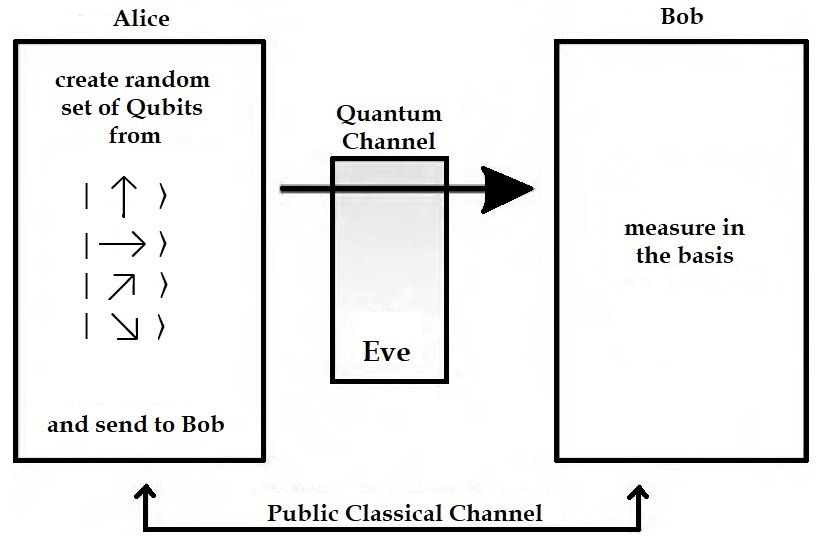
\includegraphics[width=0.8\textwidth,height=7cm]{./sdf/bb84_with_discrete_variables/figures/QKD_Model.png}
	\caption{Basic QKD Model. Alice and Bob are connected by 2 communication channels, quantum and classical, with an eavesdropper, Eve, in the quantum communication channel (figure adapted from \cite{iqo}).}\label{fig:qkd model}
\end{figure}

We are going to analyse the BB84 protocol with bit encoding into photon state polarization. Two non-orthogonal basis are used to encode the information, the rectilinear and diagonal basis, + and x respectively. The following table shows this bit encoding.
\begin{table}[H]
	\centering
	\begin{tabular}{c|c|c}
		 Bit &  \textbf{\textit{Rectilinear Basis,+}} & \textbf{\textit{Diagonal Basis,$\times$}}\\ \hline
		0 &  0$º$ & -45$º$ \\
		1 & 90$º$ & 45$º$\\
	\end{tabular}
\end{table}

The protocol is implemented with the following steps:
\begin{enumerate}
	\item Alice generates two random bit strings. The random string , $R_{A1}$, corresponds to the data to be encoded into photon state polarization. $R_{A2}$ is a random string in which 0 and 1 corresponds to the rectilinear, +, and diagonal, $\times$, respectively.
	
	$$ R_{A1} = \{0,1,1,0,1,0,0,1,1,0,1,1,1,0,0,1,0,0,0,1\}$$
	\begin{eqnarray}
		R_{A2} = \{0,0,1,0,1,1,1,0,1,1,1,0,1,0,0,0,1,0,1,0\} \\
		= \{+,+,\times,+,\times, \times, \times, +,\times, \times, \times,+,\times,+,+,+,\times,+,\times,+\}
	\end{eqnarray}
	
	\item Alice transmits a train of photons, $S_{AB}$, obtained by encoding the bits, $R_{A1}$ with the respective photon polarization state $R_{A2}$.
	
	$$S_{AB} = \{\to, \uparrow, \searrow, \to, \searrow, \nearrow, \nearrow, \uparrow, \searrow, \nearrow, \searrow, \uparrow, \searrow, \to, \to, \uparrow, \nearrow, \to, \nearrow, \uparrow\}.$$
	
	\item Bob generates a random string, $R_{B}$, to receive the photon trains with the correspondent basis.
	\begin{eqnarray}
	R_{B} = \{0,1,1,1,0,1,0,0,1,1,0,0,1,1,0,0,1,1,0,0\} \\
	=\{+,\times,\times,\times,+,\times,+,+,\times,\times,+,+,\times,\times,+,+,\times,\times,+,+\}.
	\end{eqnarray}
	
	\item Bob performs the incoming photon states measurement, $M_{B}$, with its generated random basis, $R_{B}$. If the two photon detectors don't click, means the bit was lost during transference due to attenuation. If both photon detectors click, a false positive was detected. In the measurements, $M_{B}$, the no-click in both detectors is represented by a -1 and the false positives to -2. The measurements done in rectilinear or diagonal basis are represented by 0 and 1, respectively. This is represented \ref{fig:bb84 detector}
	
	$$M_{B} = \{0,1,1,1,-1,1,0,0,-2,1,0,0,-2,1,0,0,1,-1,0,0\}$$	
	
	\begin{figure}[H]
		\centering
		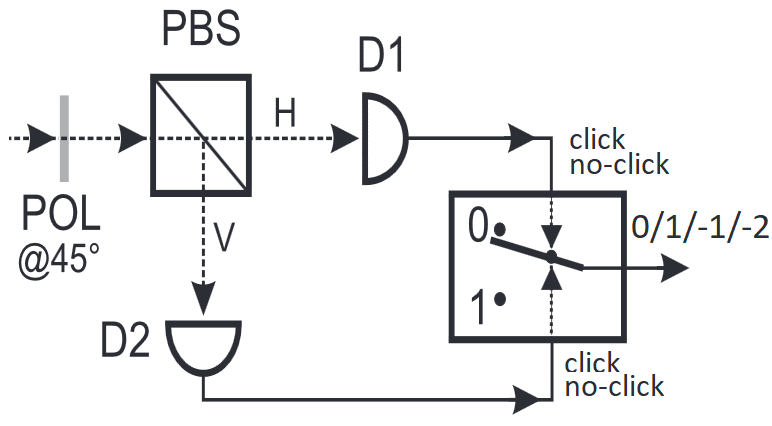
\includegraphics[width=0.8\textwidth,height=7cm]{./sdf/bb84_with_discrete_variables/figures/detector.png}
		\caption{Photon Detection block with false-positives, -2, and attenuation, -1, detection depending on D1 and D2 output.\label{fig:bb84 detector}}
	\end{figure}
	
\end{enumerate}

\textbf{Esta parte está muito confusa, preciso que o professor me explique melhor}	
The second phase, uses the classical communication channel:
\begin{enumerate}

	\item After the measurement, Bob sends to Alice the values of $M_{B}$
	\item Alice remove the bits from $R_{A2}$ corresponding to -1 and -2, performs a negated XOR, generating the bit sequence $B_{B}$ with correspondent key as $K_{A}$.
	
  	$$ K_{A} = \{0,1,0,1,0,1,0,1,0,1\}.$$
	
	\begin{table}[H]
		\centering
		\begin{tabular}{c|c c c c c c c c c c c c c c c c}
			$R_{A2}$ & 0 & 0 & 1 & 0 & 1 & 1 & 0 & 1 & 1 & 0 & 0 & 0 & 0 & 1 & 1 & 0 \\
			$R_{B}$  & 0 & 1 & 1 & 1 & 1 & 0 & 0 & 1 & 0 & 0 & 1 & 0 & 0 & 1 & 0 & 0 \\ \hline
			$B_{A}$ & 1 & 0 & 1 & 0 & 1 & 0 & 1 & 1 & 0 & 1 & 0 & 1 & 1 & 1 & 0 & 1 \\ 
		\end{tabular}
	\end{table}
	
	\item Perform a scrambling over $B_{B}$ using a known algorithm by Alice and Bob to accomplish distribute the error over all key to later and avoid error burst. Later, this will permit to have a good bit error rate estimation \cite{SPREADING}. As a example, the even positions of the $B_{B}$ will be shifted 2 positions.
	\begin{tabular}{c|c c c c c c c c c c c c c c c c}
		$Positions$ & 0 & 1 & 2 & 3 & 4 & 5 & 6 & 7 & 8 & 9 & 10 & 11 & 12 & 13 & 14 & 15 \\
		$B_{A}$  & 0 & 1 & 1 & 1 & 1 & 0 & 0 & 1 & 0 & 0 & 1 & 0 & 0 & 1 & 0 & 0 \\ 
		$P_{A}$  & 0 & 1 & 1 & 1 & 0 & 0 & 0 & 1 & 1 & 0 & 0 & 0 & 0 & 1 & 0 & 0 \\
	\end{tabular}
			
	
	\item For Bob to also have the same information, he will perform the same steps, 2 and 3 as Alice and the Key will be deduced.  $K_{AB}$
	
  	$$ K_{AB} = \{0,1,0,1,0,1,0,1,0,1\}.$$
		
\end{enumerate}

	To determine the Quantum Bit Error Rate (QBER), it is necessary some input parameters such as:
	
	\begin{enumerate}
		\item qLB - QBER lower bound.
		\item qUB - QBER upper bound.
		\item qLim - acceptable QBER limit.
	\end{enumerate}

	Then to verify if the channel is reliable or not, the flowchart presented in figure \ref{fig:flowQber}.
	
	\begin{enumerate}
		\item Bob will reveals a bit sequence from the deduced key, $K_{AB}$ to Alice. 
		\item Alice then returns to Bob the estimated QBER value, mQBER, with a confidence interval, [qLB, qUB] using the using the equations in the Bit Error Rate section, but applied to this protocol
		\item To check if the channel is compromised or not it is necessary to check if the QBER limit is higher than the QBER upper bound. If QBER limit is between the QBER lower and upper bound it is necessary to reveal more bits from the key. Otherwise the channel is compromised and the key determination process needs to restart. 
	\end{enumerate}
	
	
\begin{figure}[H]
	\centering
	\includegraphics[width=1\textwidth,height=7cm]{./sdf/bb84_with_discrete_variables/figures/qberEstimation.png}
	\caption{Flowchart to determine if the channel is reliable or not.}\label{fig:flowQber}
\end{figure}



\subsection{Simulation Setup}



\begin{figure}[H]
	\centering
	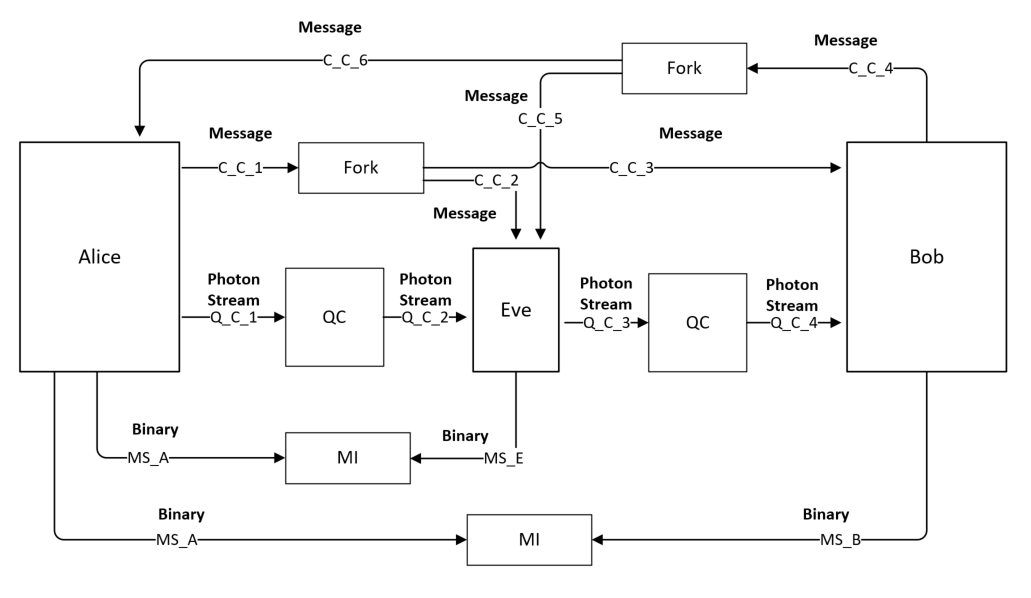
\includegraphics[width=1.0\textwidth, height=9cm]{./sdf/bb84_with_discrete_variables/figures/toplevel_simulation.png}
	\caption{Simulation diagram at a top level}\label{toplevelsimulation}
\end{figure}

Figure \ref{toplevelsimulation} presents the top level diagram of our simulation. The setup contains three parties, Alice, Eve and Bob where the communication between them is done throughout two classical and one quantum channel. In the middle of the classical channel there is a Fork's diagram which has one input and two outputs. In the case of the classical channel \textbf{C\_C\_4} which has the information sent by Bob, the fork's block enables Alice and Eve have access to it. In the quantum communication, the information sent by Alice can be intercepted by Eve and changed by her, or can follow directly to Bob as we can see later in figure \ref{evesimulation}. Furthermore, for mutual information calculation there must be two blocks \textbf{MI}, one to calculate the mutual information between Alice and Eve, and other to calculate the mutual information between Alice and Bob.

\begin{figure}[h]
	\centering
	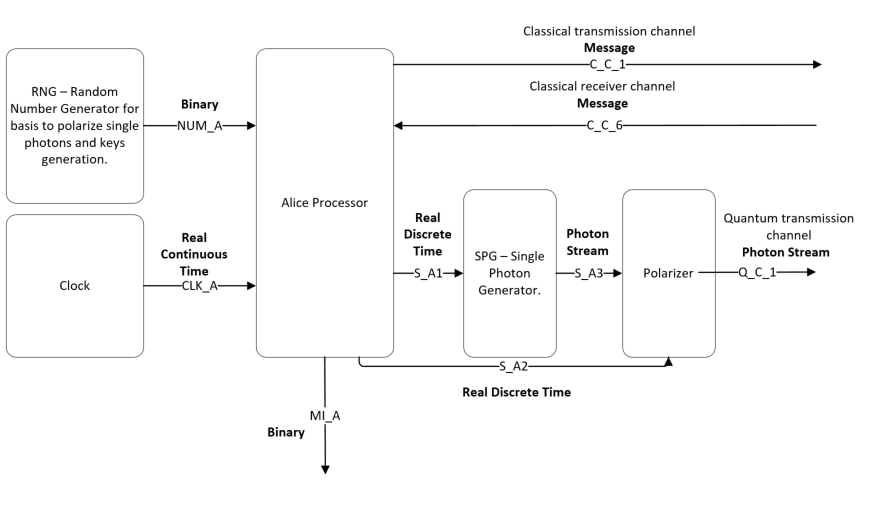
\includegraphics[width=1.0\textwidth, height=9cm]{./sdf/bb84_with_discrete_variables/figures/alice_simulation.png}
	\caption{Simulation diagram at Alice's side}\label{alicesimulation}
\end{figure}

\begin{figure}[h]
	\centering
	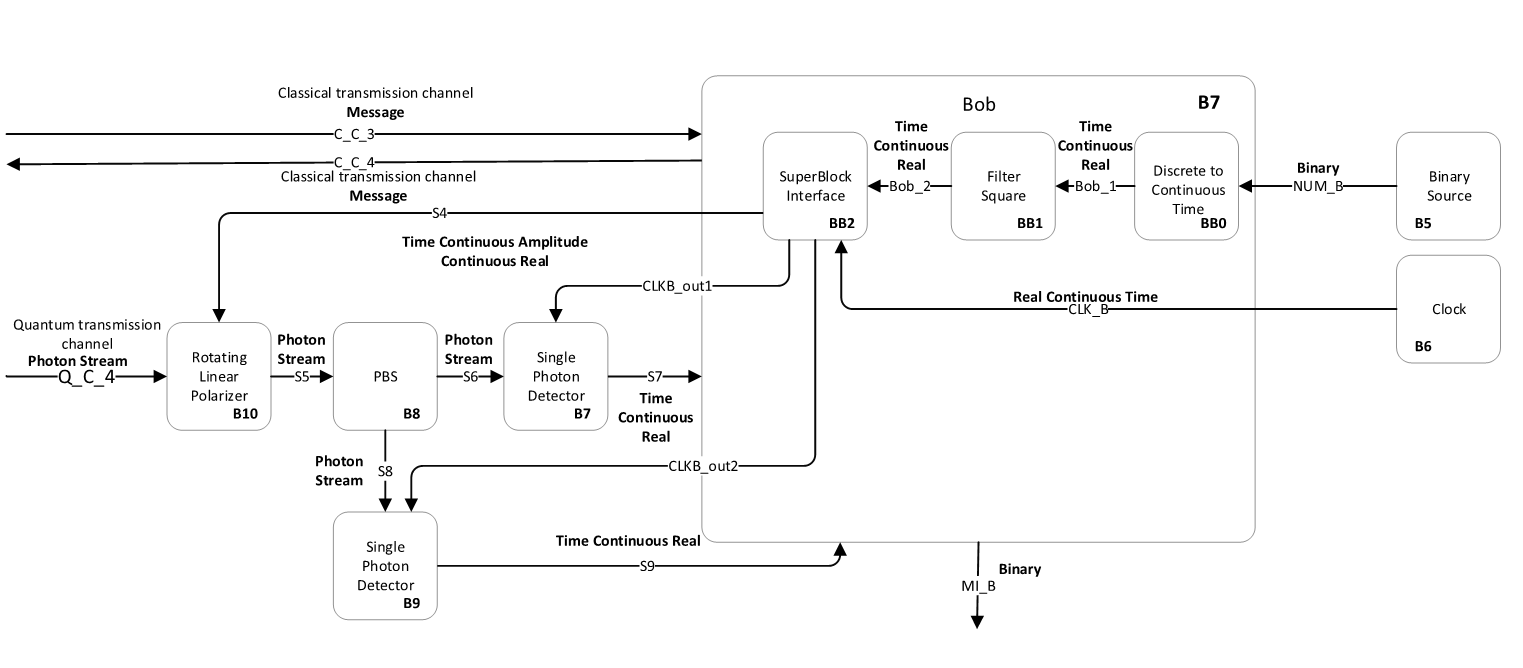
\includegraphics[width=1.0\textwidth, height=9cm]{./sdf/bb84_with_discrete_variables/figures/bob_simulation.png}
	\caption{Simulation diagram at Bob's side}\label{bobsimulation}
\end{figure}

    In figure \ref{alicesimulation} one can observe a block diagram of the simulation at Alice's side. As it is shown in the figure, Alice must have one block for random number generation which is responsible for basis generation to polarize the photons, and for key random generation in order to have a random state to encode each photon. Furthermore, she has a Processor block for all logical operations: array analysis, random number generation requests, and others. This block also receives the information from Bob after it has passed through a fork's block. In addition, it is responsible for set the initial length $l$ of the first array of photons which will send to Bob. This block also must be responsible for send classical information to Bob. Finally, Processor block will also send a real continuous time signal to single photon generator, in order to generate photons according to this signal, and finally this block also sends to the polarizer a real discrete signal in order to inform the polarizer which basis it should use. Therefore, she has two more blocks for quantum tasks: the single photon generator and the polarizer block which is responsible to encode the photons generated from the previous block and send them throughout a quantum channel from Alice to Bob.

    Finally, Alice's processor has an output to Mutual Information top level block, $Ms_{A}$.

     In figure \ref{bobsimulation} one can observe a block diagram of the simulation at Bob's side. From this side, Bob has one block for Random Number Generation which is responsible for randomly generate basis values which Bob will use to measure the photons sent by Alice throughout the quantum channel. Like Alice, Bob has a Processor block responsible for all logical tasks, analysing functions, requests for random number generator block, etc. Additionally, it receives information from Alice throughout a classical channel after passed through a fork's block and a quantum channel. However, Bob only sends information to Alice throughout a classical channel. Furthermore, Bob has one more block for single photon detection which receives from processor block a real discrete time signal, in order to obtain the basis it should use to measure the photons.

    Finally, Bob's processor has an output to Mutual Information top level block, $Ms_{B}$.



\begin{figure}[h]
	\centering
	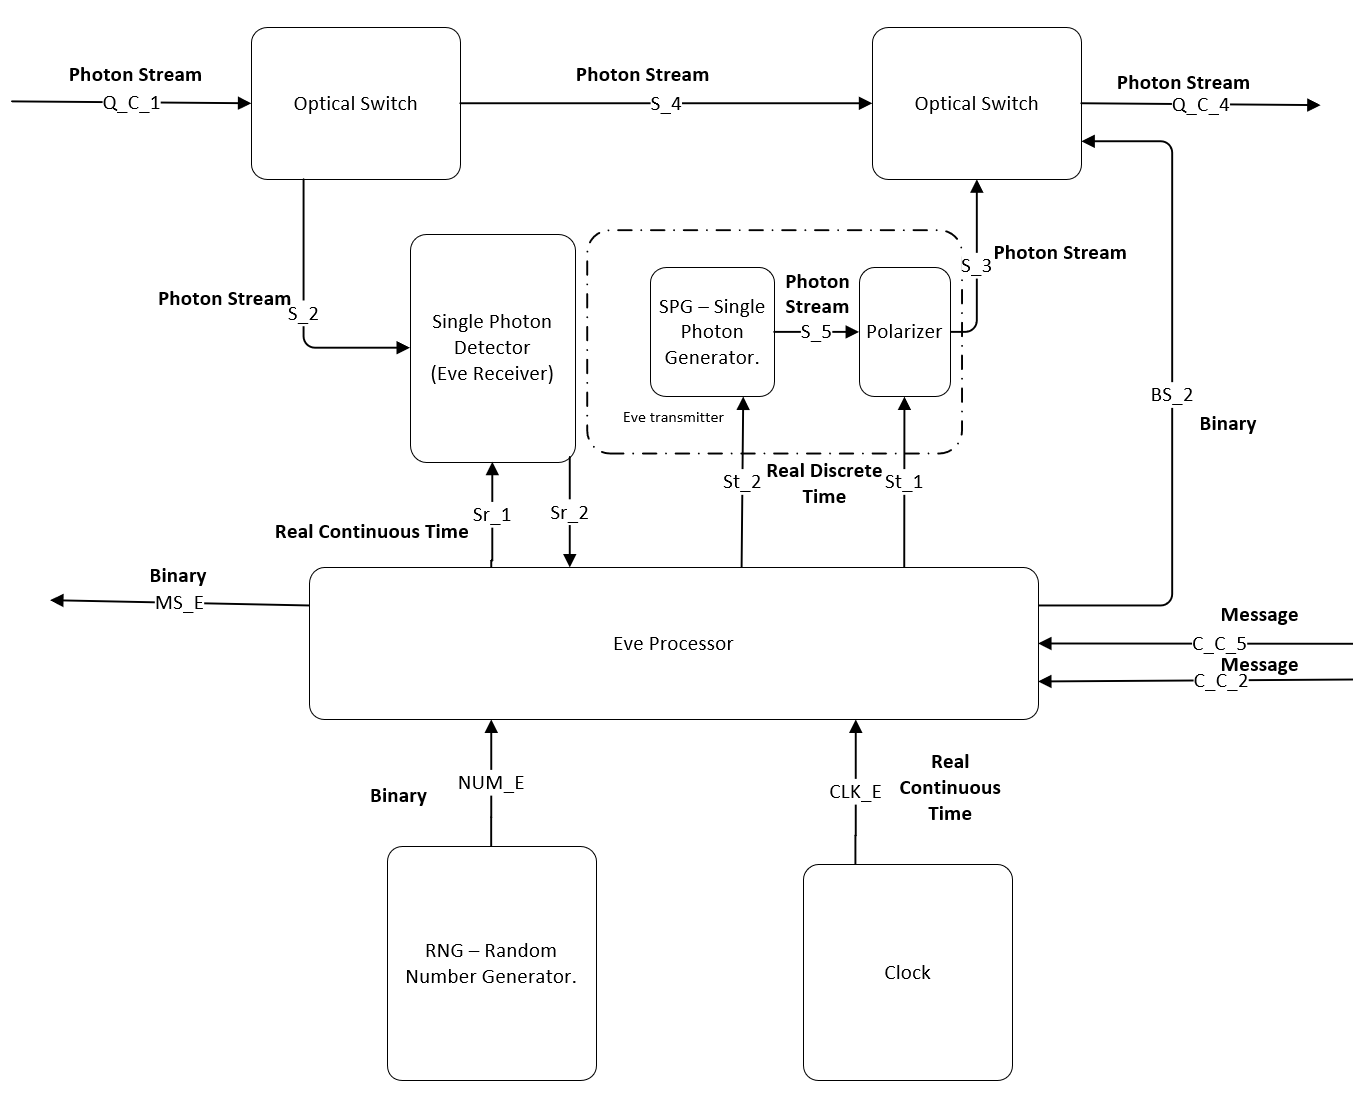
\includegraphics[width=1.1\textwidth, height=14cm]{./sdf/bb84_with_discrete_variables/figures/eve_simulation.png}
	\caption{Simulation diagram at Eve's side}\label{evesimulation}
\end{figure}

Figure \ref{evesimulation} presents the Eve's side diagram. Eve's processor has two receiver classical signals, one from Alice (\textbf{C\_C\_2}) and other from Bob (\textbf{C\_C\_5}). About quantum channel, Eve received a quantum message from Alice through the channel \textbf{Q\_C\_1} and depends on her decision the photon can follows directly to Bob or the photon's state can be changed by her. In this case, the photon is received by a block similar to Bob's diagram \ref{bobsimulation} and this block sends a message to Eve's processor in order to reveal the measurement result. After that, Eve's processor sends a message to Alice's diagram similar to figure \ref{alicesimulation} and this block is responsible for encode the photon in a new state. Now, the changed photon is sent to Bob.

In addition, Eve's diagram has one more output $Ms_{E}$ which is a message sent to the mutual information block as an input parameter.

\begin{table}[hbt]
\centering
\caption{System Signals}
\label{tb:signals}
\begin{tabular}{|c|c|c|}
\hline
\textbf{Signal name}         & \textbf{Signal type} & \textbf{Status} \\ \hline
C\_C\_1 ... C\_C\_6          & Message              &                 \\ \hline
Q\_C\_1 .. Q\_C\_4           & Photon Stream        &                 \\ \hline
Ms\_A, Ms\_B, Ms\_E          & Binary               &                 \\ \hline
NUM\_A , NUM\_B, NUM\_E      & Binary               &                 \\ \hline
CLK\_A, CLK\_B, CLK\_E       & Real continuous time &                 \\ \hline
SB\_1, SB\_2, Sr\_1, Sr\_2   & Real continuous time &                 \\ \hline
SA\_1, SA\_2, St\_1, St\_2   & Real discrete time   &                 \\ \hline
SA\_3                        & Photon  Stream       &                 \\ \hline
S\_2, S\_3, S\_4, S\_5       & Photon Stream        &                 \\ \hline
BS\_1, BS\_2                 & Binary               &                 \\ \hline
\end{tabular}
\end{table}

Table \ref{tb:signals} presents the system signals as well as them type.

\begin{table}[hbt]
\centering
\caption{System Input Parameters}
\label{tb:inputparameters}
\begin{tabular}{|c|c|c|}
\hline
\textbf{Parameter}           & \textbf{Default Value}                           & \textbf{Description} \\ \hline
SymbolRate                   & 100K                                             &                 \\ \hline
NumberOfBits                 & Number of photons that Alice sends to Bob        &                 \\ \hline

\end{tabular}
\end{table}

\begin{table}[hbt]
\centering
\caption{Header Files}
\label{tb:signals}
\begin{tabular}{|c|c|c|}
\hline
\textbf{File name}              & \textbf{Description} & \textbf{Status} \\ \hline
binary\_source.h       &                      &                 \\ \hline
single\_photon\_source.h      &                      &                 \\ \hline
single\_photon\_detector.h       &                      &                 \\ \hline
optical\_switch.h                       &                      &       Missing          \\ \hline
polarization\_beam\_splitter.h                       &                      &                 \\ \hline
mutual\_information.h            &                      &            Missing     \\ \hline
bit\_error\_rate.h                       &                      &                 \\ \hline
clock.h                       &                      &                 \\ \hline
fiber.h                       &                      &                 \\ \hline
qrng\_decision\_circuit.h                       &                      &                 \\ \hline
message\_to\_send.h               &                      &      Missing           \\ \hline
message\_to\_receive.h            &                      &      Missing           \\ \hline
netxpto.h                       &                      &                 \\ \hline
\end{tabular}
\end{table}

\begin{table}[hbt]
\centering
\caption{Source Files}
\label{tb:signals}
\begin{tabular}{|c|c|c|}
\hline
\textbf{File name}              & \textbf{Description} & \textbf{Status} \\ \hline
binary\_source.cpp       &                      &                 \\ \hline
single\_photon\_sourcer.cpp      &                      &                 \\ \hline
single\_photon\_detector.cpp       &                      &                 \\ \hline
optical\_switch.cpp                       &                      &   Missing              \\ \hline
polarization\_beam\_splitter.cpp                       &                      &                 \\ \hline
mutual\_information.cpp            &                      &       Missing          \\ \hline
bit\_error\_rate.cpp            &                      &                 \\ \hline
clock.cpp            &                      &                 \\ \hline
fiber.cpp            &                      &                 \\ \hline
qrng\_decision\_circuit.cpp            &                      &                 \\ \hline
message\_to\_send.cpp               &                      &       Missing          \\ \hline
message\_to\_receive.cpp            &                      &       Missing          \\ \hline
netxpto.cpp                       &                      &                 \\ \hline
bb84\_sdf.cpp                       &                      &                 \\ \hline
\end{tabular}
\end{table} 

\begin{thebibliography}{2}
	\bibitem{BB84} 
	Bennett, C. H. and Brassard,
	G. Quantum Cryptography: Public key distribution and coin tossing.
	International Conference on Computers, Systems and Signal Processing, Bangalore, India, 10-12 December 1984, pp. 175-179.
	
	\bibitem{SURV}
	Mart Haitjema, A Survey of the Prominent Quantum Key Distribution Protocols
	
	\bibitem{iqo}
	Christopher Gerry, Peter Knight, "Introductory Quantum Optics" Cambridge University Press, 2005
	
	\bibitem{SPREADING}
	Varadarajan, S., Ngo, H. Q., \& Srivastava, J. (n.d.). An Adaptive , Perception-Driven Error Spreading Scheme in Continuous Media Streaming.
	
\end{thebibliography}
\cleardoublepage
